\chapter{HCI Basics}

\section{Introduction}

Human-Computer Interaction focuses on creating interfaces that are not only functional but also intuitive and accessible to users. In the context of the \textit{Birds of Sweden Dashboard}, HCI principles guide the design decisions to ensure users can effectively explore and analyze bird observation data across Sweden.

This chapter goes through how Interaction Design principles are applied.

\section{Interaction Design and the Five Dimensions}

\subsection{What is Interaction Design?}

Interaction Design (IxD) is the discipline of designing interactive products and services with a focus on how users will interact with them. It goes beyond the mere functionality of an item, considering users' needs, limitations, and contexts to tailor the experience accordingly \cite{WhatInteractionDesign2024}. This user-centered approach ensures that the design meets precise demands, facilitating seamless interaction between the user and the product.

\subsection{Application of Weber's Law and Fitts's Law}

Perceptual laws like Weber's Law and Fitts's Law play a significant role in interface design, influencing how users perceive and interact with elements.

\paragraph{Weber's Law}

Weber's Law states that the just-noticeable difference between two stimuli is proportional to the magnitude of the stimuli \cite{mccrocklinInteractionDesignData2015}. In interface design, this means that subtle differences in element sizes or colors may go unnoticed.

\paragraph{Fitts's Law}

Fitts's Law predicts that the time required to move to a target area is a function of the distance to the target and the size of the target \cite{mccrocklinInteractionDesignData2015}. Smaller targets that are farther away are harder and slower to click.

\paragraph{Application to the Dashboard}

\begin{itemize}
    \item \textbf{Hoverability of Data Points}: Initially, small scatter points on the map made it difficult for users to hover over and click them, violating Fitts's Law. 
    \item \textbf{Improvement Implemented}: By adding \texttt{hovermode='closest'} to the scatter mapbox, the interactive area around each data point (cursor bubble) was increased. 
    \item \textbf{Benefits}: 
    \begin{itemize} 
        \item \textbf{Easier Interaction}: Users do not need to precisely hover over tiny points, reducing the effort and time required. 
        \item \textbf{Enhanced Accessibility}: Larger interactive areas assist users with motor impairments or those using touch devices. 
    \end{itemize} 
\end{itemize}

\begin{figure}[H] 
    \centering 
    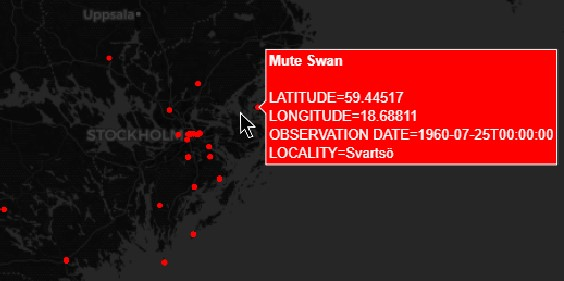
\includegraphics[width=0.6\textwidth]{figures/cursor_bubbles.jpg} 
    \caption{Tooltip displayed if cursor is near a data point.} 
    \label{fig:cursor_bubbles} 
\end{figure}

\subsection{The Five Dimensions of Interaction Design}

Gillian Crampton Smith and Kevin Silver defined five dimensions that interaction designers consider when designing interactions \cite{WhatInteractionDesign2024}:

\begin{enumerate} 
    \item \textbf{Words (1D)}: Text elements like button labels that provide necessary information to users. 
    \item \textbf{Visual Representations (2D)}: Graphical elements such as images, typography, and icons that aid user interaction. 
    \item \textbf{Physical Objects/Space (3D)}: The medium through which users interact with the product, like a mouse, keyboard, or touch screen. 
    \item \textbf{Time (4D)}: Media that change over time, including animations, videos, and sounds. 
    \item \textbf{Behavior (5D)}: How the previous dimensions define the interactions a product affords, including user actions and system reactions. 
\end{enumerate}

Interaction designers utilize these dimensions to consider interactions holistically, envisioning real-world user demands for designs not yet introduced.

\subsection{Application to the Birds of Sweden Dashboard}

The \textit{Birds of Sweden Dashboard} incorporates the five dimensions of interaction design to enhance user experience:

\paragraph{Words (1D)}

The dashboard uses clear and concise text to guide users:

\begin{itemize} 
    \item \textbf{Button Labels and Dropdown Options}: The species selection dropdown is labeled "Select a species," providing a straightforward instruction. 
    \item \textbf{Informational Text}: The sidebar displays species names, scientific names, and additional details, ensuring users understand the information presented. 
\end{itemize}

\paragraph{Visual Representations (2D)}

Graphical elements are employed to facilitate understanding:

\begin{itemize} 
    \item \textbf{Maps}: The main map and the state observations map visually represent bird observations geographically. 
    \item \textbf{Images}: Species images retrieved from Wikipedia help users visually identify birds. 
    \item \textbf{Icons and Typography}: Consistent use of fonts and styling enhances readability and aesthetic appeal. 
\end{itemize}

\paragraph{Physical Objects/Space (3D)}

Users interact with the dashboard through various physical mediums:

\begin{itemize} 
    \item \textbf{Mouse}: Primary interaction for clicking, hovering, and navigating the map. 
    \item \textbf{Keyboard}: Supports navigation through the dropdown and accessibility features. 
    \item \textbf{Touch Devices}: Basic touch interactions are possible, though optimization is needed. 
\end{itemize}

\paragraph{Time (4D)}

Temporal elements enhance the interactive experience:

\begin{itemize} 
    \item \textbf{Interactive Map Updates}: The map dynamically updates when a species is selected, providing immediate feedback. 
    \item \textbf{Hover Effects}: Tooltips appear when hovering over data points, offering additional information. 
\end{itemize}

\paragraph{Behavior (5D)}

The dashboard's behavior defines user interactions:

\begin{itemize} 
    \item \textbf{User Actions}: Selecting species, zooming the map, and clicking on data points are intuitive actions supported. 
    \item \textbf{System Reactions}: The dashboard responds to user inputs by updating visuals and information displayed, reinforcing progress toward user goals. 
\end{itemize}

\section{Cognitive Walkthrough}

A cognitive walkthrough was performed using Rick Spencer's \textit{Streamlined Cognitive Walkthrough Method} \cite{spencerStreamlinedCognitiveWalkthrough2000} to evaluate the dashboard's usability. The walkthrough focuses on typical tasks that users might perform. It aims to assess whether the interface supports these tasks effectively.

\subsection{Users and Tasks}

\paragraph{User Profile}

The primary users are:

\begin{itemize} 
    \item \textbf{Bird Enthusiasts}: Individuals interested in birdwatching and bird data exploration. 
    \item 
    \textbf{Ornithologists and Researchers}: Professionals studying bird patterns and behaviors. 
    \item \textbf{Conservationists}: Individuals involved in wildlife conservation efforts. 
\end{itemize}

\paragraph{Selected Tasks}

Four key tasks were identified:

\begin{enumerate} 
    \item Explore the overall distribution of bird observations. 
    \item Find information about a specific bird species. 
    \item Identify regions where a selected species is commonly observed. 
    \item View detailed information about a specific observation. 
\end{enumerate}

\subsection{Action Sequences and Walkthrough Analysis}

The action sequences are presented on the left, with the corresponding walkthrough on the right.

\subsubsection{Task 1: Explore Overall Distribution of Bird Observations}

\begin{table}[H]
    \centering
    \begin{tabular}{p{0.45\textwidth} | p{0.5\textwidth}}
        \hline
        \textbf{Action Sequence} & \textbf{Walkthrough Analysis} \\
        \hline
        \begin{enumerate}
            \item Open the dashboard.
            \item Observe the initial map displaying all observations.
        \end{enumerate} &
        \begin{itemize}
            \item \textbf{Will the user know what to do?} Yes; the map is immediately visible upon opening the dashboard.
            \item \textbf{Will the user know they are making progress?} Yes; the dense distribution of data points indicates active observations.
        \end{itemize} \\
        \hline
    \end{tabular}
    \caption{Cognitive Walkthrough for Task 1}
    \label{tab:task1_walkthrough}
\end{table}

\subsubsection{Task 2: Find Information About a Specific Bird Species}

\begin{table}[H]
    \centering
    \begin{tabular}{p{0.45\textwidth} | p{0.5\textwidth}}
        \hline
        \textbf{Action Sequence} & \textbf{Walkthrough Analysis} \\
        \hline
        \begin{enumerate}
            \item Locate the species dropdown in the sidebar.
            \item Click on the dropdown to view options.
            \item Type or scroll to find the desired species.
            \item Select the species from the list.
        \end{enumerate} &
        \begin{itemize}
            \item \textbf{Step 1}: The dropdown is labeled and prominently placed, so users will know what to do.
            \item \textbf{Step 2}: Clicking the dropdown is a common interaction.
            \item \textbf{Step 3}: Users can type to search or scroll through the list.
            \item \textbf{Step 4}: Upon selection, the map and sidebar update, so users know they are making progress.
        \end{itemize} \\
        \hline
    \end{tabular}
    \caption{Cognitive Walkthrough for Task 2}
    \label{tab:task2_walkthrough}
\end{table}

\subsubsection{Task 3: Identify Regions Where the Selected Species is Commonly Observed}

\begin{table}[H]
    \centering
    \begin{tabular}{p{0.45\textwidth} | p{0.5\textwidth}}
        \hline
        \textbf{Action Sequence} & \textbf{Walkthrough Analysis} \\
        \hline
        \begin{enumerate}
            \item Observe the main map after species selection.
            \item Note the distribution of observation points.
            \item Look at the state observations map in the sidebar.
        \end{enumerate} &
        \begin{itemize}
            \item \textbf{Step 1}: The map is the focal point, so users know what to do.
            \item \textbf{Step 2}: Clusters indicate regions with frequent observations, helping users track progress.
            \item \textbf{Step 3}: The sidebar map provides a choropleth view. Color intensities reflect observation counts, so users understand their progress.
        \end{itemize} \\
        \hline
    \end{tabular}
    \caption{Cognitive Walkthrough for Task 3}
    \label{tab:task3_walkthrough}
\end{table}

\subsubsection{Task 4: View Detailed Information About a Specific Observation}

\begin{table}[H]
    \centering
    \begin{tabular}{p{0.45\textwidth} | p{0.5\textwidth}}
        \hline
        \textbf{Action Sequence} & \textbf{Walkthrough Analysis} \\
        \hline
        \begin{enumerate}
            \item Hover over a data point on the main map.
            \item Click on the data point.
            \item Observe any additional information displayed.
        \end{enumerate} &
        \begin{itemize}
            \item \textbf{Step 1}: Users may naturally hover, but tooltips might not be expected if points are small.
            \item \textbf{Step 2}: Clicking is not immediately obvious; a prompt could help.
            \item \textbf{Step 3}: The sidebar updates, but additional visual feedback (e.g., animation) would improve the experience.
        \end{itemize} \\
        \hline
    \end{tabular}
    \caption{Cognitive Walkthrough for Task 4}
    \label{tab:task4_walkthrough}
\end{table}